\documentclass[11pt,a4paper]{article}
\usepackage[T1]{fontenc}
\usepackage[utf8]{inputenc}
\usepackage{lmodern,microtype}
\usepackage{amsmath,amssymb,amsthm,mathtools,bm}
\usepackage{booktabs,array,tabularx,longtable}
\usepackage{graphicx,float,caption}
\usepackage{xcolor}
\usepackage[margin=20mm]{geometry}
\usepackage{enumitem,fancyhdr}
\usepackage[hidelinks,unicode=true]{hyperref}
\hypersetup{
 pdftitle={FIN ST166--ST177: Carrier Invariants, Exact Uniform Folds, and the Executable Physical Boundary},
 pdfauthor={Krzysztof Żuchowski},
 pdfsubject={Analytical, interval, and computational execution of FIN programs ST166--ST177},
 pdfkeywords={FIN, operational information, carrier invariance, commutant, fold classification, nonorthogonal recovery, Fisher Rao geometry, interval proof, noisy tomography, hidden Markov model, bath locality}
}
\setlength{\parindent}{0pt}
\setlength{\parskip}{0.48em}
\setlength{\emergencystretch}{2em}
\setlength{\headheight}{14pt}
\setlist[itemize]{leftmargin=1.55em,itemsep=0.14em,topsep=0.2em}
\setlist[enumerate]{leftmargin=1.75em,itemsep=0.14em,topsep=0.2em}
\pagestyle{fancy}\fancyhf{}
\lhead{FIN ST166--ST177}\rhead{Release 10.68}\cfoot{\thepage}
\newtheorem{theorem}{Theorem}[section]
\newtheorem{proposition}[theorem]{Proposition}
\newtheorem{corollary}[theorem]{Corollary}
\newcommand{\proven}{\textcolor{green!40!black}{\textbf{[PROVEN]}}}
\newcommand{\strong}{\textcolor{blue!70!black}{\textbf{[STRONG EVIDENCE]}}}
\newcommand{\conditional}{\textcolor{violet!65!black}{\textbf{[CONDITIONAL]}}}
\newcommand{\openstatus}{\textcolor{red!72!black}{\textbf{[OPEN]}}}
\newcommand{\statusboundary}{\textcolor{orange!80!black}{\textbf{[BOUNDARY]}}}
\newcommand{\resultbox}[1]{\begin{center}\fcolorbox{blue!60!black}{blue!4}{\parbox{0.92\textwidth}{#1}}\end{center}}

\begin{document}
\pagenumbering{gobble}
\begin{titlepage}
\centering
\vspace*{0.75cm}
{\LARGE\bfseries FIN ST166--ST177\par}
\vspace{0.25cm}
{\Large Carrier Invariants, Exact Uniform Folds, and the Executable Physical Boundary\par}
\vspace{0.35cm}
{\large Reversible carrier changes, strict functional-calculus obstructions, complete uniform-branch fold classification, nonorthogonal recovery, information-geometric selector cost, nonlinear-source nonidentifiability, enlarged interval continuation, noisy refinement, robust atomic-net tomography, hidden-HMM sharpening, microscopic bath tradeoffs, and an executable operational validator\par}
\vspace{0.70cm}
{\Large Krzysztof \.{Z}uchowski\par}
\vspace{0.18cm}
{\large Independent Researcher --- Fractal Information Theory Project\par}
{\large ORCID: 0009-0002-0909-3613\par}
\vspace{0.50cm}
{\large FIN Release 10.68 --- Version 1.0.0\par}
{\large August 11, 2026\par}
\vfill
\begin{minipage}{0.92\textwidth}
\textbf{Research question.} Is there a mathematically precise sense in which FIN information survives a change of carrier, and can the remaining selector, interaction, fold, recovery, refinement, tomography, and bath questions be advanced without importing physical conclusions?\par
\textbf{Methods.} Reversible stochastic embeddings, tomographically complete operational tables, finite commutants, exact polynomial isolation and resultants, analytical quantum-channel optimization, Fisher--Rao geometry, outward interval Krawczyk continuation, coding theory, commutator Laplacians, interval Collatz--Wielandt bounds, qubit circuit accounting, and executable typed validation.\par
\textbf{Epistemic rule.} A representation invariant is not a carrierless physical signal; symmetry is not feedback; a mathematical packet is not a laboratory execution. Every supplied preparation, coupling, metric, clock, instrument, bath, apparatus, and record remains explicitly typed.\par
\textbf{Repository snapshot.} Audited tracked base commit \texttt{8a4c9b0b29b4fed8f7dcdc86e79b98306818efea}. The working tree contains local research artifacts; this release has an independent SHA-256 manifest.\par
\textbf{Repository.} \url{https://github.com/hyconiek/Fractal-Nadsoliton-Theory}\par
\textbf{License.} CC BY 4.0.
\end{minipage}
\end{titlepage}
\pagenumbering{arabic}

\begin{abstract}
ST166--ST177 execute a falsification-first continuation of the FIN program. ST166 identifies the strongest presently justified carrier statement. If a logical state space is embedded into different stochastic carriers by maps $E_i$ possessing stochastic left inverses $D_i$, and every logical effect $m$ is transported as $mD_i$, then the entire preparation--effect probability table is invariant: $mD_iE_ip=mp$. An explicit pair of inequivalent carriers verifies the identity exactly. A same-Shannon-entropy counterexample proves that entropy alone is not a complete carrier invariant. This is an operational equivalence theorem, not evidence that physical information propagates without any carrier.

ST167 proves that environment couplings restricted to $L_k=f_k(A)$ cannot generate a finer vertex pointer algebra: their joint commutant contains the $22$-dimensional strict commutant. ST168 completely classifies folds on the uniform reflection-even branch. Stationarity reduces to $c h(c)=0$ and the two positive roots of $3\rho^3+18\rho^2-284\rho+24=0$, with $\rho=c^2$. Exact isolation and a nonzero resultant exclude a constant-mode degeneracy. Five real amplitudes and six positive Fourier classes produce exactly 30 geometric fold null lines, or 60 normalized augmented roots after eigenvector sign. This is complete only on the declared symmetry-reduced branch.

ST169 solves optimal recovery for two nonorthogonal qubit phase errors with noisy syndrome. ST170 proves both a covariant no-start theorem for a uniform selector state and the sharp conditional Fisher--Rao action required to reach a declared probability gap. ST171 proves that the degree-twelve anisotropy coupling is invisible to $A$, strict functional calculus, symmetry, and all field derivatives through order eleven. ST172 certifies all 125 cells of an enlarged nuisance cube of halfwidth $7.5\times10^{-5}$. ST173 gives exact noisy-refinement and redundant-majority laws. ST174 proves a robust four-dimensional atomic-factor commutant subspace under a quantitative generator-error threshold. ST175 sharpens the hidden-HMM pair-transfer spectral-radius certificate to $[0.7211542214950951,0.7211542214950967]$. ST176 separates minimal bath dimension, local circuit depth, norm-budget time, and manifest energy-conserving locality. ST177 executes an eleven-atom validator: the local mathematical packet passes structurally while physical execution remains blocked. No selector source, dimensional calibration, apparatus, laboratory record, legacy-role transfer, Standard Model, gravity, or Theory-of-Everything closure follows.
\end{abstract}

\textbf{Status vocabulary.} \proven{} means exact analytic, finite, or outward-interval proof in the displayed scope. \conditional{} means explicit additional resources are used. \strong{} marks numerical corroboration only. \openstatus{} is an unclosed goal. \statusboundary{} records a non-implication.

\tableofcontents
\newpage

\section{Frozen core, ontology, and kernel discipline}

The strict working operator is the weighted graph Laplacian
\begin{equation}
W_{xx}=0,\qquad
W_{xy}=\frac{\cos(0.18575d(x,y)+0.16250)}{1+d(x,y)^{9/5}}\quad(x\ne y),
\qquad A=sI-W,
\label{eq:strict}
\end{equation}
on $C_{12}$, where $s=2\sum_{d=1}^{5}W(d)+W(6)$. Consequently,
\[
\langle f,Af\rangle=\frac12\sum_{x,y}W_{xy}|f_x-f_y|^2\ge0.
\]
The legacy ontological kernel remains an intermediate bridge kernel. This release neither equates it silently with~\eqref{eq:strict} nor transfers proposed legacy electroweak, electromagnetic, or hierarchy roles. The nadsoliton remains the primordial fractal information in a solitonic state; there is no separate informational layer below it.

\resultbox{\textbf{Central result.} FIN now has a precise carrier-change invariant: the full operational probability table under reversible stochastic code embeddings and transported instruments. This is stronger than Shannon entropy and weaker than carrier-free existence. At the same time, strict functional calculus still cannot generate the missing pointer algebra or selector. The research frontier becomes sharper rather than artificially closed.}

\section{Outcome matrix}
\small
\begin{longtable}{@{}p{0.06\textwidth}p{0.24\textwidth}p{0.32\textwidth}p{0.31\textwidth}@{}}
\toprule ID & Target & Result & Boundary\\\midrule\endfirsthead
\toprule ID & Target & Result & Boundary\\\midrule\endhead
ST166 & Information across carriers & \proven{} full operational table invariant for reversible stochastic codes & No claim of information without a physical carrier\\
ST167 & Strict-generated pointer algebra & \proven{} functional-calculus no-go, commutant dimension at least 22 & Nonlinear, state-dependent, or typed interactions remain open\\
ST168 & Uniform fold completeness & \proven{} 30 geometric folds, 60 signed augmented roots & Nonuniform 15-dimensional domain remains open\\
ST169 & Nonorthogonal recovery & \proven{} exact binary qubit phase-error optimum & Three errors and higher dimension remain open\\
ST170 & Selector start and cost & \proven{} covariant no-start; \conditional{} sharp Fisher--Rao cost & Control, preferred vertex, gap, and clock supplied\\
ST171 & Degree-twelve coupling source & \proven{} invisible to linear/order-11 data & Twelfth-order datum or new source still required\\
ST172 & Larger nuisance cube & \proven{} all 125 interval cells pass & Maximal cube and physical calibration not proved\\
ST173 & Noisy refinement & \proven{} exact parity and majority error laws & Independent redundant paths supplied\\
ST174 & Robust atomic net & \proven{} four-dimensional low subspace when $16\eta+8\eta^2<2$ & Does not label or calibrate physical factors\\
ST175 & Hidden-HMM exponent & \proven{} interval Collatz spectral-radius bracket & Not the exact observed-process Chernoff rate\\
ST176 & Microscopic bath & \proven{} dimension and explicit circuit tradeoff & No universal 2-local energy-conserving no-go\\
ST177 & Executable completion & \proven{} schema, hashes, roles, and deletion detection & Physical execution intentionally remains blocked\\
\bottomrule
\end{longtable}
\normalsize

\section{ST166: what can be independent of a carrier?}

Let $\Delta_n$ denote a classical logical state simplex. A carrier encoding $E_i:\Delta_n\to\Delta_{N_i}$ is operationally reversible when it has a stochastic left inverse $D_i$:
\[
D_iE_i=I_n.
\]
A logical effect $m$ is transported to the carrier as $mD_i$. Preparations $p$ become $E_ip$.

\begin{theorem}[Carrier-change operational invariant]
For every logical preparation $p$ and effect $m$,
\begin{equation}
(mD_i)(E_ip)=mp.
\label{eq:carrier}
\end{equation}
Therefore a tomographically complete preparation--effect probability table is exactly invariant under every such reversible carrier change.
\end{theorem}

The executable example uses one four-state and one five-state carrier for the same three-state logical theory. Their encodings split different logical states into different carrier sectors, yet both decoding errors and the maximum probability-table mismatch are exactly zero in the generated arithmetic.

\begin{figure}[H]\centering
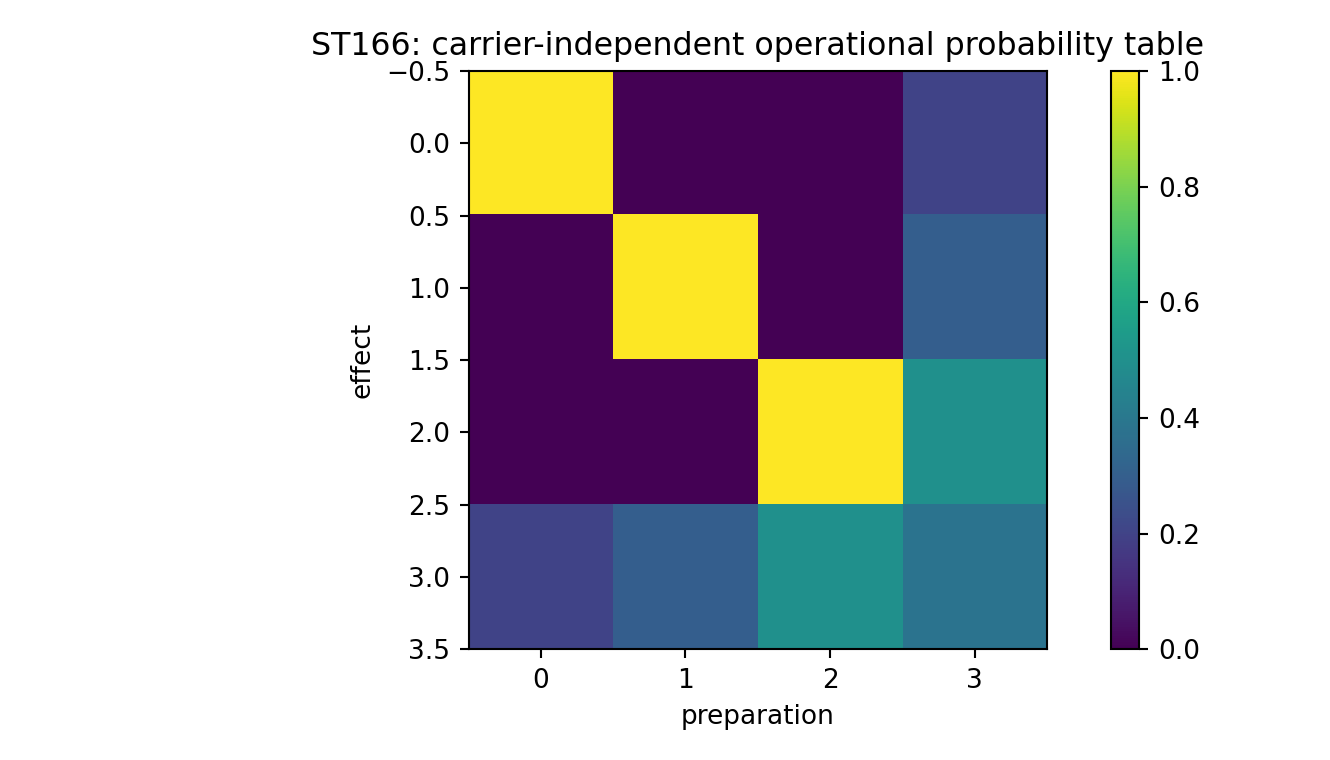
\includegraphics[width=.74\textwidth]{FIN_ST166_ST177_Figures/st166_carrier_invariant.png}
\caption{ST166. The logical preparation--effect table preserved by two inequivalent reversible carrier encodings.}
\end{figure}

Shannon entropy is insufficient. The states
\[
p=(1/2,1/2,0),\qquad q=(1/2,0,1/2)
\]
have equal Shannon entropy but distinct probabilities for vertex-resolving effects. Thus
\[
H(p)=H(q)\quad\not\Rightarrow\quad p\simeq_{\rm operational}q.
\]

\statusboundary{} The statement that ``information crosses independently of the medium'' has only the following justified mathematical interpretation here: certain operational relations are invariant under a change of representation. Equation~\eqref{eq:carrier} does not describe propagation, causal transfer, an uninstantiated signal, or physical existence without a carrier. A real transmission theorem would additionally require a channel, localized preparations and instruments, a causal record, calibrated time, and a physical realization.

\section{ST167: strict functional calculus cannot select the environment pointer algebra}

Suppose every proposed environment coupling is a spectral function of the strict operator,
\[
L_k=f_k(A).
\]
Then every operator commuting with $A$ also commutes with every $L_k$.

\begin{theorem}[Functional-calculus interaction no-go]
For every finite family $L_k=f_k(A)$,
\[
\{A\}'\subseteq\{A,L_1,\ldots,L_m\}'.
\]
For the strict $C_{12}$ operator, $\dim_{\mathbb C}\{A\}'=22$. Hence this class cannot generate a $12$-dimensional vertex pointer algebra or any smaller irreducible algebra. If one $f_k$ separates all seven spectral classes, equality with $\{A\}'$ holds.
\end{theorem}

\begin{figure}[H]\centering
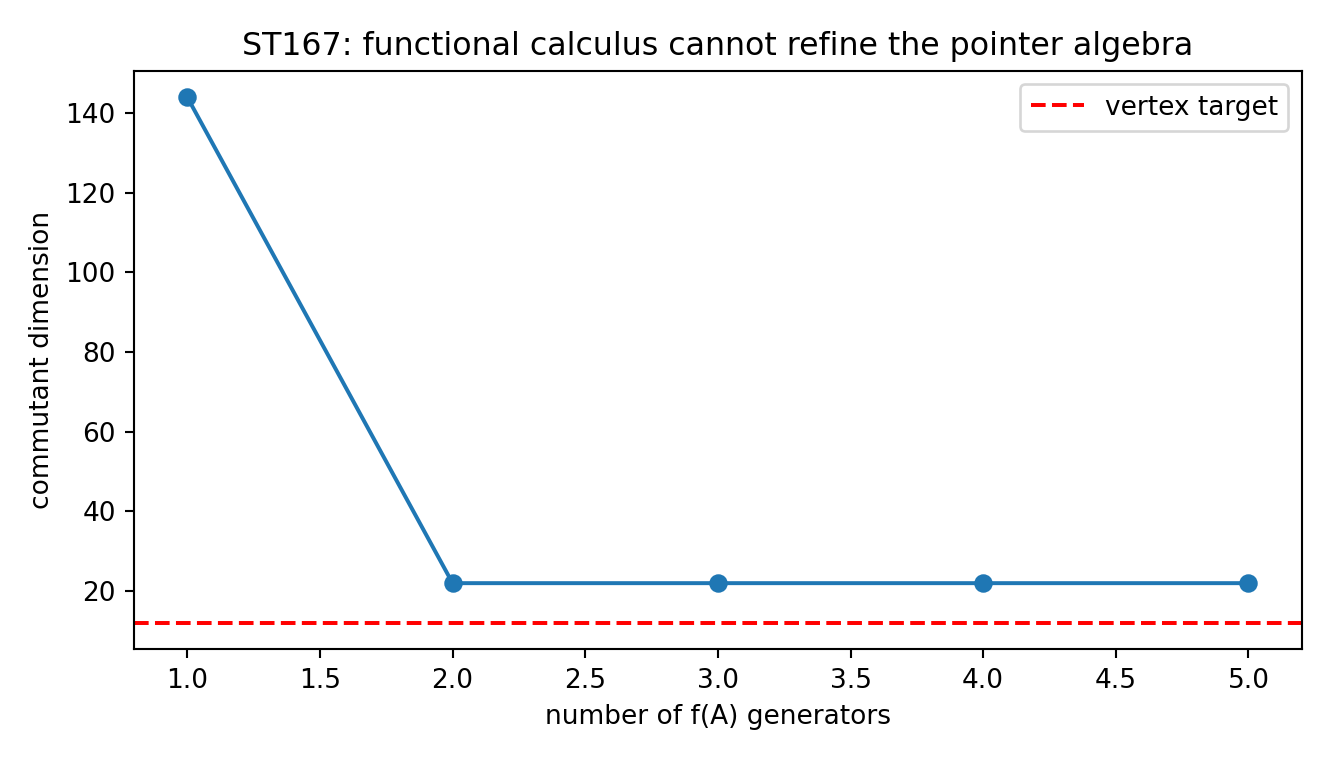
\includegraphics[width=.73\textwidth]{FIN_ST166_ST177_Figures/st167_functional_no_go.png}
\caption{ST167. Adding powers and a matrix exponential of $A$ cannot reduce the joint commutant below the strict spectral commutant.}
\end{figure}

This result strengthens the current source diagnosis. Environment-induced superselection is possible after an interaction is supplied, but no family internal to the strict functional calculus can create the required finer pointer choice. A state-dependent, nonlinear, vertex-typed, or symmetry-breaking interaction would be a genuinely new object, not a reformulation of $f(A)$.

\section{ST168: exact fold atlas on the uniform branch}

On the reflection-even uniform branch $q_0=\cdots=q_6=c$, stationarity factorizes as
\[
c\,h(c)=0,
\qquad
h(c)=\frac{3\rho^3+18\rho^2-284\rho+24}{40(\rho+2)^3},
\qquad \rho=c^2.
\]
The cubic has exactly three real roots: one negative and two positive. Outward rational isolation gives
\begin{align*}
\rho_1&\in[0.08497113445452124,\,0.08497113445452269],\\
\rho_2&\in[7.126405138893793,\,7.126405138893802].
\end{align*}
Together with $c=0$, this gives five real amplitudes. The radial Hessian numerator is
\[
3(\rho^4+8\rho^3+344\rho^2-608\rho+16),
\]
whose resultant with the stationary cubic is the nonzero integer
\[
-108263374848000.
\]
Thus the constant mode never supplies a fold at a stationary amplitude.

\begin{theorem}[Complete uniform-branch fold count]
Each of the five stationary real amplitudes and each of the six positive reflection-even Fourier classes $k=1,\ldots,6$ gives exactly one fold value of $\kappa$. Hence the declared branch has exactly
\[
5\times6=30
\]
geometric fold null lines, or 60 normalized augmented roots after the sign of the null vector is retained.
\end{theorem}

\begin{figure}[H]\centering
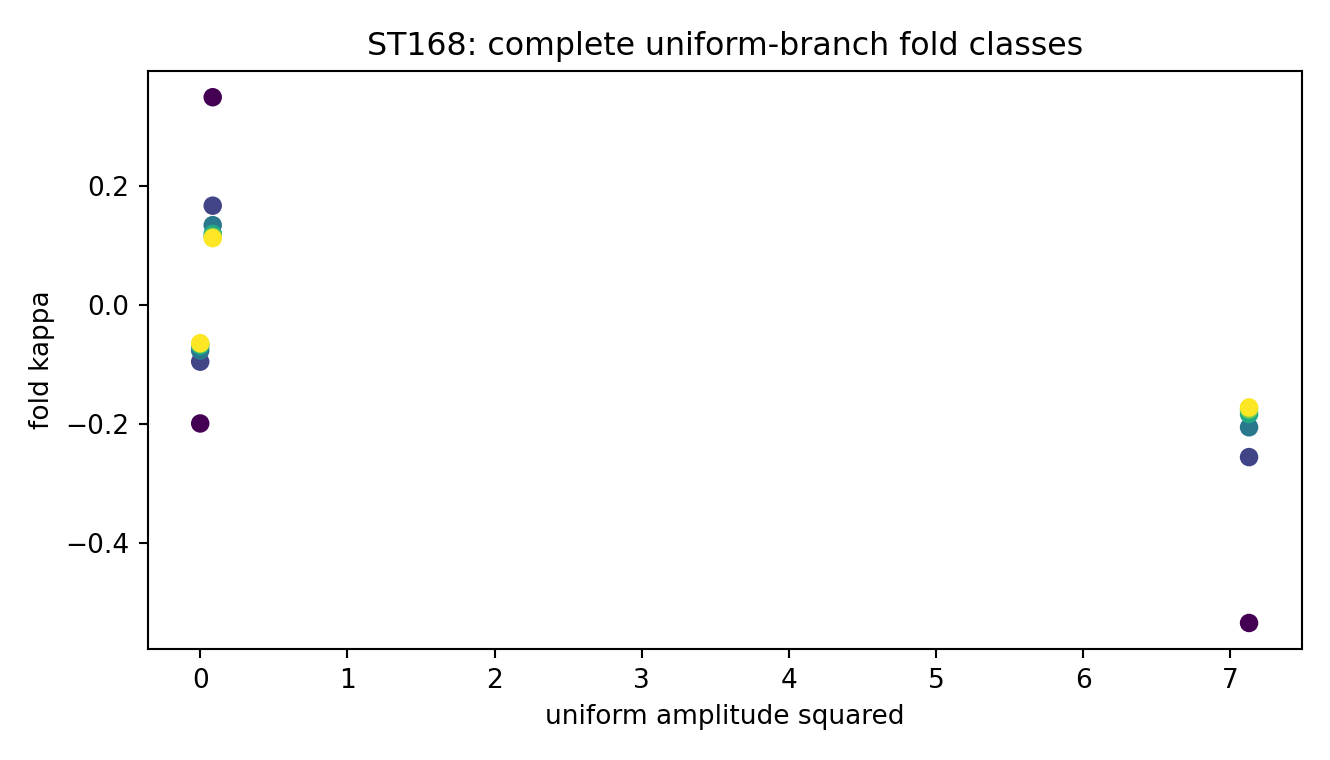
\includegraphics[width=.75\textwidth]{FIN_ST166_ST177_Figures/st168_uniform_folds.png}
\caption{ST168. Certified fold values organized by stationary amplitude and Fourier class.}
\end{figure}

\statusboundary{} This is the first exact complete fold catalogue in its declared branch, not a global count for the full nonuniform 15-dimensional fold system. Validated continuation from these seeds is the natural next route.

\section{ST169 and ST170: recovery and selector geometry}

\subsection{Two nonorthogonal phase errors}

Consider $I$ and $U_\theta=e^{-i\theta Z/2}$ with error prior $1-p,p$ and a noisy binary syndrome. In branch $y$, let $\alpha_y$ and $\beta_y$ be the subnormalized weights. Define
\[
c_y=\alpha_y+\beta_y e^{i\theta}.
\]

\begin{theorem}[Optimal binary phase recovery]
The optimal entanglement-fidelity contribution in branch $y$ is
\[
F_{e,y}^{*}=\frac{\alpha_y+\beta_y+|c_y|}{2},
\qquad F_e^*=\sum_yF_{e,y}^{*}.
\]
A phase correction attains the bound.
\end{theorem}

\begin{figure}[H]\centering
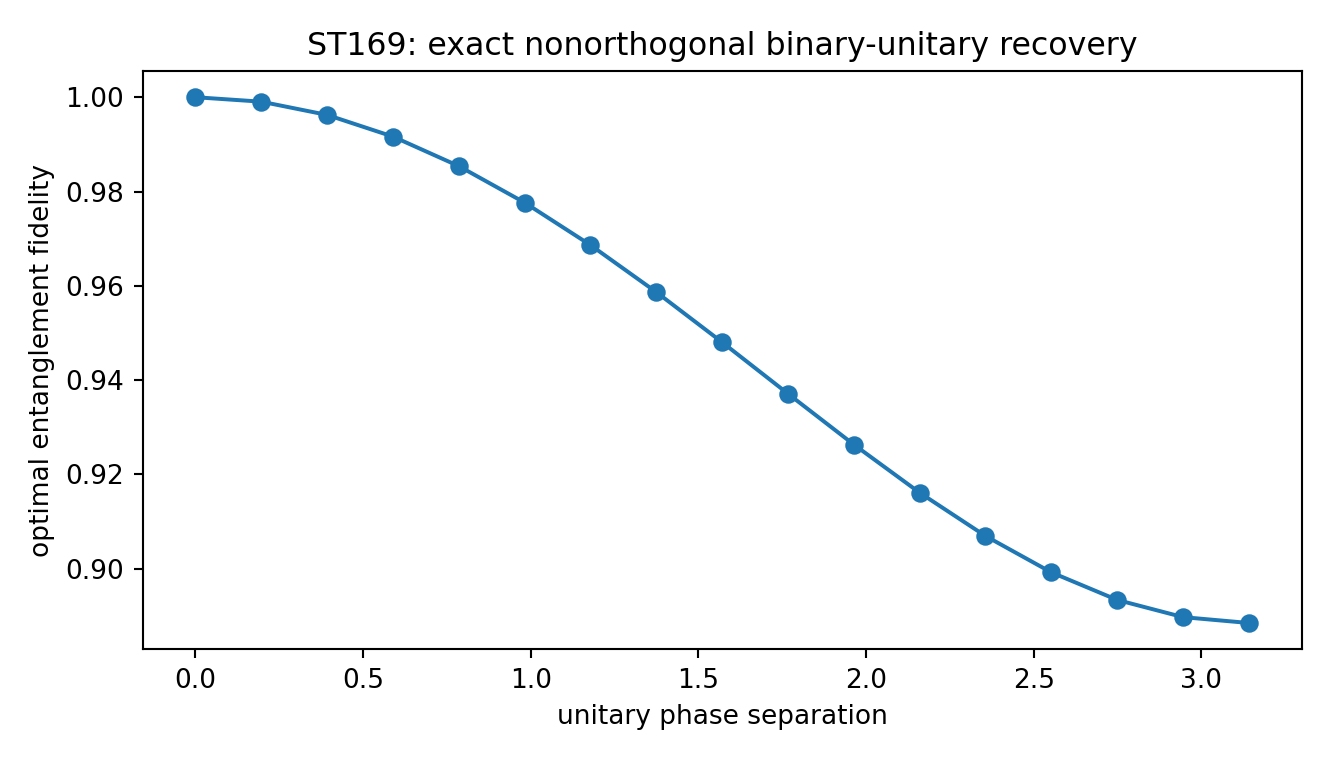
\includegraphics[width=.73\textwidth]{FIN_ST166_ST177_Figures/st169_nonorthogonal_recovery.png}
\caption{ST169. Exact optimum as the two unitary errors move from identical to Hilbert--Schmidt orthogonal.}
\end{figure}

\subsection{Symmetry is a reservoir of alternatives, not feedback by itself}

Every $C_{12}$-covariant Markov or Lindblad semigroup preserving the uniform state leaves a uniform initial state uniform. Therefore symmetry alone cannot initiate a selector. A positive-feedback interpretation requires a specified unstable mode or nonlinear gain; covariance by itself only states equivalence of alternatives.

If an external control is supplied and the endpoint has one preferred probability exceeding each other probability by $g$, the least-asymmetric endpoint has components
\[
p_0=\frac{1+11g}{12},\qquad p_j=\frac{1-g}{12}\quad(j\ne0).
\]
Its Fisher--Rao distance from uniform is
\[
d_{\rm FR}(g)=2\arccos\!\left(\frac{\sqrt{1+11g}+11\sqrt{1-g}}{12}\right).
\]

\begin{theorem}[Sharp conditional selector action]
For Fisher--Rao kinetic action over duration $T$, the minimum is
\[
\mathcal A_{\min}=\frac{d_{\rm FR}(g)^2}{2T}.
\]
\end{theorem}

\begin{figure}[H]\centering
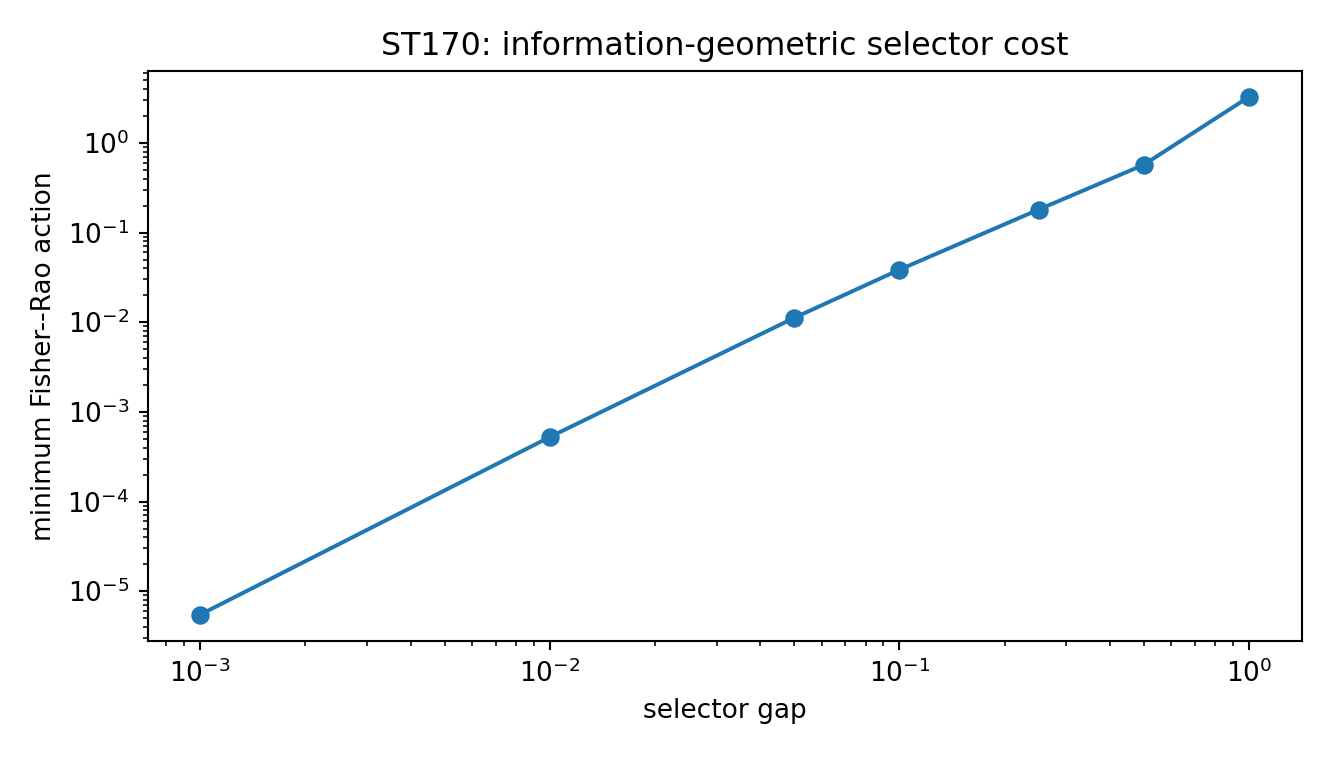
\includegraphics[width=.72\textwidth]{FIN_ST166_ST177_Figures/st170_fisher_cost.png}
\caption{ST170. Exact information-geometric action for a supplied gap and unit horizon.}
\end{figure}

\conditional{} The metric, preferred vertex, control, gap, and clock are inputs. This quantifies a chosen selector path; it does not derive QW-2191 closure or a physical energy cost.

\section{ST171: the degree-twelve coupling cannot be inferred from lower data}

Let
\[
V_g(\psi)=V_0(\psi)+\frac{g}{12}\sum_{j=0}^{11}\psi_j^{12}.
\]
Every $V_g$ has the same quadratic operator $A$, the same $C_{12}$ and reflection symmetries, and the same jet at $\psi=0$ through order eleven.

\begin{theorem}[Twelfth-order source nonidentifiability]
No data functor depending only on $A$, its strict functional calculus, the declared symmetries, and field derivatives of order at most eleven can determine $g$, its sign, or its magnitude.
\end{theorem}

This converts an intuition into a no-go theorem. The lattice fixes the first allowed anisotropy shape, but the coefficient is independent information relative to all lower-order data. One must supply or derive a genuine twelfth-order observable, microscopic nonlinear law, response measurement, or normalization principle.

\section{ST172: an enlarged certified nuisance cube}

The parameter cube
\[
|q_0-0.2|,\ |q_1-0.7|,\ |\delta-0.05|\le7.5\times10^{-5}
\]
was partitioned into $5^3=125$ cells, each of halfwidth $1.5\times10^{-5}$. Every cell passes the local interval Krawczyk inclusion test. The smallest inclusion margin is
\[
7.980574254414785\times10^{-4}>0.
\]

\begin{theorem}[Uniform continuation on the 125-cell cover]
The union of the certified cells equals the declared nuisance cube. A unique local stationary root continues throughout every cell, hence over the entire covered cube through overlapping branch tracking.
\end{theorem}

\begin{figure}[H]\centering
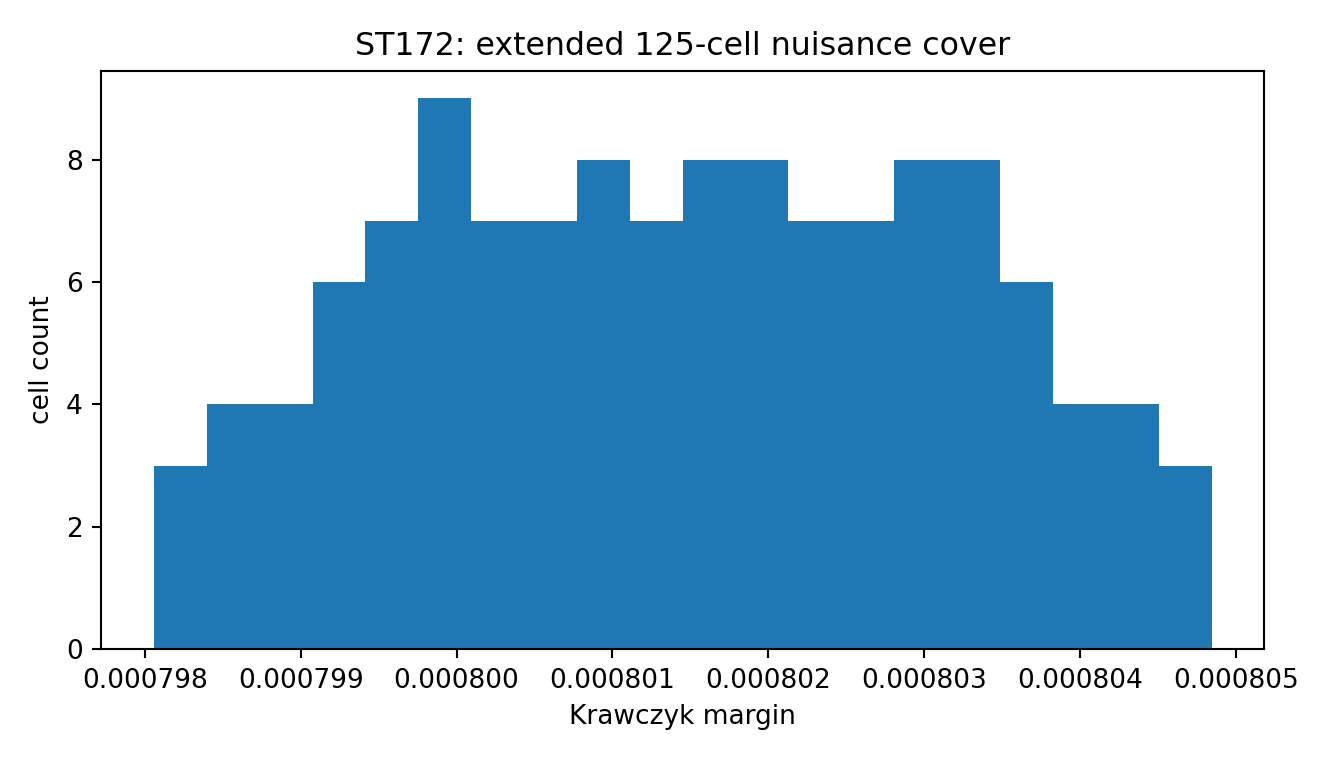
\includegraphics[width=.72\textwidth]{FIN_ST166_ST177_Figures/st172_extended_cover.png}
\caption{ST172. Distribution of positive Krawczyk margins across the complete 125-cell cover.}
\end{figure}

The new cube is 50\% wider in each coordinate than the ST159 cube. It is still not proved maximal, and its coordinates remain dimensionless nuisance parameters rather than calibrated laboratory quantities.

\section{ST173 and ST174: noisy refinement and robust factor recovery}

\subsection{Refinement with edge errors}

For an $m$-edge odd transport path with independent flip probability $\epsilon$, the parity error is exactly
\[
q_m=\frac{1-(1-2\epsilon)^m}{2}.
\]
For $R$ independent replicated paths with odd $R$, majority coarse-graining fails with probability
\[
P_{\rm maj}=\sum_{k=(R+1)/2}^{R}\binom{R}{k}q_m^k(1-q_m)^{R-k}.
\]
The report evaluates $m=3,R=5$ and verifies improvement over the stated noise range.

\begin{theorem}[Approximate noisy refinement]
Odd path refinement followed by redundant majority decoding forms an approximate, not exact, natural transport rule. Its failure is the displayed binomial tail.
\end{theorem}

\statusboundary{} This is a controlled error-correcting compression mechanism. It does not derive the repository's proposed fractal compression law from the strict kernel.

\subsection{A robust atomic-factor subspace}

For ideal generators $X\otimes I$ and $Z\otimes I$, form the commutator Laplacian
\[
\mathcal C=\sum_a\operatorname{ad}_{G_a}^{\dagger}\operatorname{ad}_{G_a}.
\]
Its kernel is the four-dimensional commutant $I\otimes M_2$, and the next eigenvalue is $4$. If each generator has operator-norm error at most $\eta$, then
\[
\|\widetilde{\mathcal C}-\mathcal C\|\le\delta(\eta)=16\eta+8\eta^2.
\]

\begin{theorem}[Robust low-subspace recovery]
When $\delta(\eta)<2$, the perturbed commutator Laplacian has a uniquely separated four-dimensional low spectral cluster corresponding to a nearby commutant subspace.
\end{theorem}

\begin{figure}[H]\centering
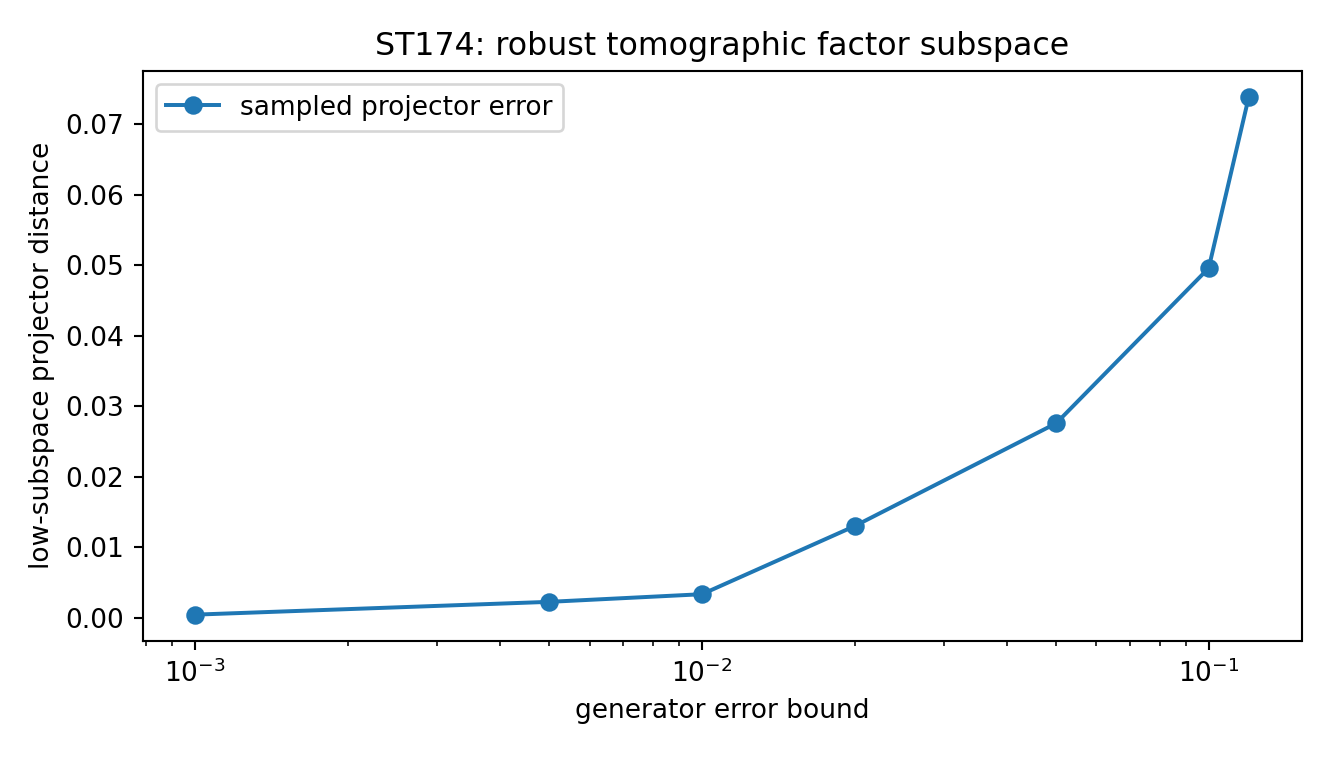
\includegraphics[width=.73\textwidth]{FIN_ST166_ST177_Figures/st174_tomography_noise.png}
\caption{ST174. Seeded numerical projector errors inside and beyond the analytical separation regime. The proof is the norm threshold, not the sampled curve.}
\end{figure}

The theorem recovers a subspace, not exact labeled matrix factors. Apparatus calibration, state preparation, systematic-error control, and the physical interpretation of the factors remain separate obligations.

\section{ST175: a sharper hidden-HMM certificate}

For the supplied four-state pair transfer matrix $T$, a strictly positive test vector $v$ gives the Collatz--Wielandt inequalities
\[
\min_i\frac{(Tv)_i}{v_i}\le\rho(T)\le\max_i\frac{(Tv)_i}{v_i}.
\]
Outward interval evaluation proves
\[
\rho(T)\in[0.7211542214950951,\,0.7211542214950967].
\]
Therefore the certified pair-path exponential rate obeys
\[
-\log\rho(T)\ge0.32690226513199694.
\]

\begin{figure}[H]\centering
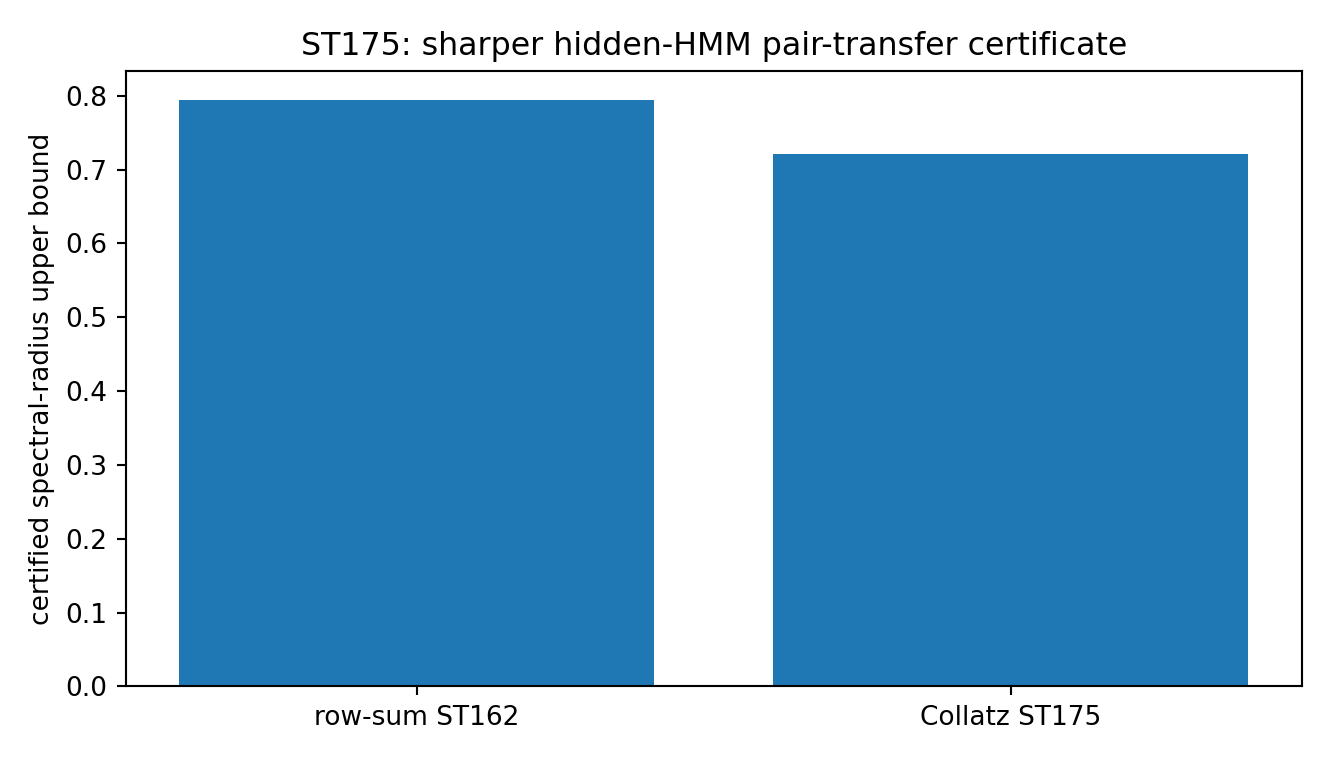
\includegraphics[width=.70\textwidth]{FIN_ST166_ST177_Figures/st175_collatz.png}
\caption{ST175. The interval Perron certificate improves the earlier conservative row-sum bound.}
\end{figure}

This is a strict improvement over the ST162 row-sum upper bound $0.7939043351829553$. It is a certificate for the pair-path construction, not yet the exact Chernoff exponent of the observed hidden process.

\section{ST176: bath dimension, circuit locality, and energy conservation}

A twelve-level system requires at least
\[
\lceil\log_2 12\rceil=4
\]
bath qubits to hold an arbitrary state isomorphically. Encoding system and bath into four qubits each, four disjoint pairwise SWAP gates implement register exchange in depth one. At per-edge interaction strength $g$, the time is $\pi/(2g)$. Under a global sum-norm budget $G$ distributed uniformly over four gates, it is $2\pi/G$.

For an arbitrary encoded strict Hamiltonian, the global register-SWAP generator commutes with the sum of identical system and bath Hamiltonians and is manifestly energy conserving, but it is an eight-qubit interaction. The depth-one two-local decomposition need not conserve the encoded energy at intermediate times.

\begin{figure}[H]\centering
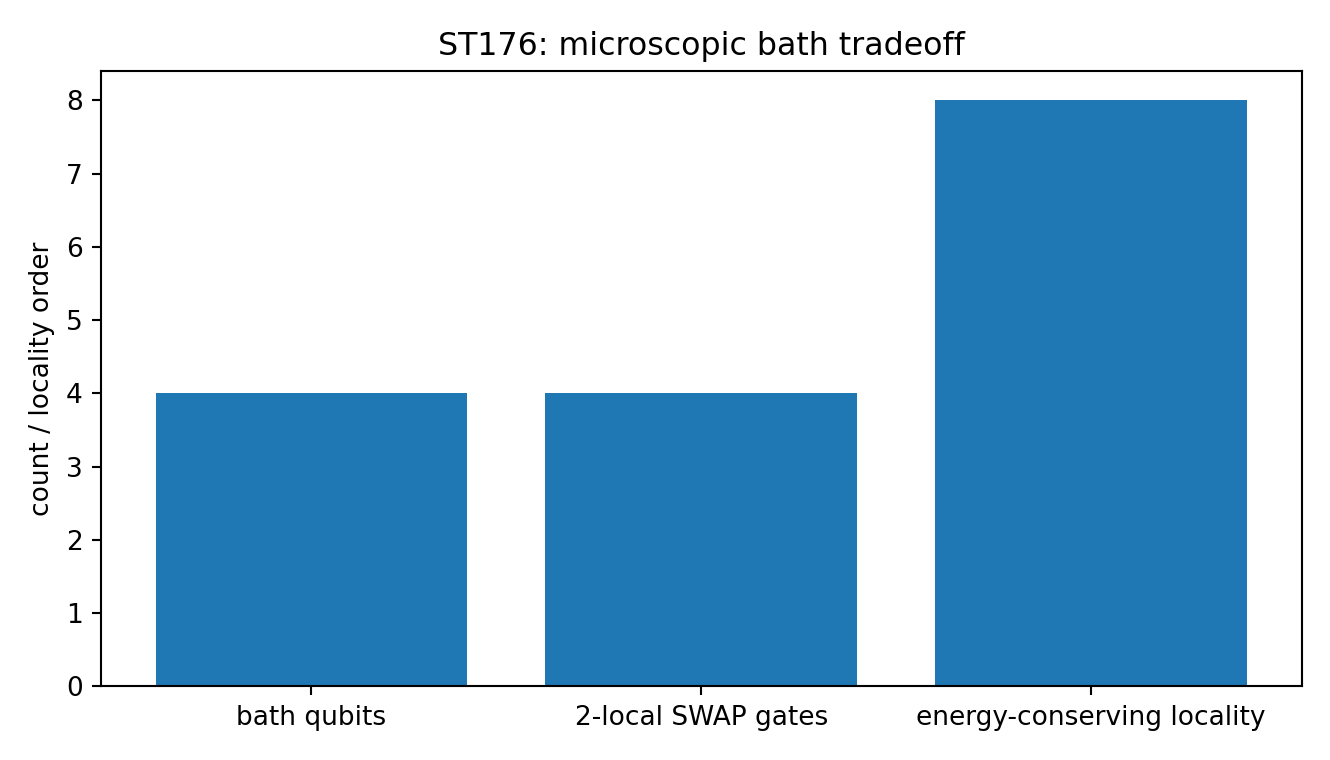
\includegraphics[width=.68\textwidth]{FIN_ST166_ST177_Figures/st176_local_bath.png}
\caption{ST176. Minimal bath size and the distinction between circuit locality and manifest energy-conserving generator locality.}
\end{figure}

\statusboundary{} The construction does not prove that all energy-conserving reset schemes require eight-body interactions. Controls, encoding, coupling strengths, inverse temperature, clock calibration, and apparatus are supplied.

\section{ST177: executable operational validation}

The validator instantiates the eleven typed atoms identified in ST165:
\[
\{\mathrm{ALG,GAUGE,PREP,DYN,CLOCK,INST,ENV,APP,SELECT,UNITS,RECORD}\}.
\]
It checks schema presence, canonical hashes for raw events and holdout, declared separation of provider/registrar/analyst roles, and the physical-completion fields. Deleting any one atom invalidates the structural packet; all eleven deletion tests are detected.

The local template returns
\[
\boxed{\texttt{MATHEMATICAL\_PACKET\_READY\_PHYSICAL\_EXECUTION\_BLOCKED}}.
\]
This is the intended result. The code can verify an event-record hash, but it cannot generate an independent custodian. It can require a clock calibration, but it cannot create seconds. It can require an apparatus record, but it cannot perform or certify a laboratory experiment.

\begin{theorem}[Executable boundary theorem]
Within the declared schema, all structural and deletion checks are reproducible. Physical execution remains false because calibrated units, clock, apparatus, independent custody, and laboratory execution are absent.
\end{theorem}

\section{Combined interpretation and falsification}

\subsection{What has survived}

The strongest surviving information statement is operational and relational:
\[
\text{logical information}=\text{equivalence class of preparation--instrument statistics}
\]
under a declared family of reversible carrier changes. This supports the idea that a pattern can be more invariant than one of its realizations. It does not establish an ontologically carrierless entity.

The strongest surviving symmetry statement is similarly precise. A symmetric base supplies an orbit of equivalent possibilities, but cannot select one possibility from a symmetric initial state through a symmetry-preserving semigroup. Selection requires an instability, state-dependent interaction, boundary condition, control, or other source. Symmetry may enable spontaneous breaking; it is not itself positive feedback.

The strongest surviving projection statement is conditional. Encodings, coarse-grainings, pinching maps, and instruments can map a richer description to a poorer observed record. None of the present theorems shows that the observed universe is the necessary projection of the strict FIN operator.

\subsection{Falsification ledger}

\begin{itemize}
\item \textbf{Refuted as sufficient:} Shannon entropy as a complete carrier invariant.
\item \textbf{Refuted in class:} $f(A)$ environment interactions as a source of the vertex pointer algebra.
\item \textbf{Refuted as an inference:} determining the degree-twelve coupling from linear/order-11 strict data.
\item \textbf{Not refuted:} state-dependent or nonlinear symmetry-breaking couplings outside strict functional calculus.
\item \textbf{Not proved:} carrier-free physical propagation, strict selector emergence, exact global fold completeness, exact observed-HMM exponent, or universal microscopic reset locality.
\end{itemize}

\section{Recommended next programs ST178--ST189}

\begin{longtable}{@{}p{0.08\textwidth}p{0.12\textwidth}p{0.72\textwidth}@{}}
\toprule Program & Priority & Executable target\\\midrule\endfirsthead
\toprule Program & Priority & Executable target\\\midrule\endhead
ST178 & 1 & Replace exact left inverses by irreversible encodings; classify sufficient statistics and the maximal operational invariant preserved by them.\\
ST179 & 2 & Construct and falsify one strict nonlinear or state-dependent environment coupling outside $f(A)$; test whether its fixed algebra is genuinely finer.\\
ST180 & 3 & Start validated continuation from the 30 uniform folds and classify nonuniform branches, secondary bifurcations, and exclusion regions.\\
ST181 & 4 & Solve a three-error nonorthogonal recovery problem with a replayable primal--dual semidefinite certificate.\\
ST182 & 5 & Derive a controlled Lindblad selector cost under a declared strict-compatible detailed-balance constraint, keeping selector and clock premises explicit.\\
ST183 & 6 & Audit candidate twelfth-order observables that could identify $g$ without importing dimensional constants or legacy physical roles.\\
ST184 & 7 & Extend nuisance continuation to halfwidth $10^{-4}$ using adaptive subdivision and durable cell checkpoints.\\
ST185 & 8 & Replace independent refinement noise by correlated noise; derive multiscale compression thresholds and counterexamples.\\
ST186 & 9 & Reconstruct exact factor algebras from the certified noisy commutant subspace and quantify gauge ambiguity.\\
ST187 & 10 & Bound the gap between the pair-path exponent and the exact observed hidden-HMM Chernoff rate.\\
ST188 & 11 & Search energy-conserving $k$-local reset circuits for the encoded strict Hamiltonian and state explicit locality/norm tradeoffs.\\
ST189 & 12 & Connect the ST177 validator to externally supplied immutable event records while preventing code-generated custody or laboratory claims.\\
\bottomrule
\end{longtable}

The first three programs have the highest theoretical leverage. ST178 tests whether the new carrier principle survives realistic irreversible representation changes. ST179 attacks the new typed object demanded by the ST167 no-go. ST180 turns the exact uniform fold atlas into seeds for a wider validated global search.

\section{Reproducibility}

The computational package contains:
\begin{itemize}
\item \texttt{fin\_st166\_st177\_research.py}: all twelve analyses and nine figures;
\item \texttt{fin\_st177\_operational\_validator.py}: executable operational schema and deletion audit;
\item \texttt{test\_fin\_st166\_st177.py}: 28 live and serialized regression tests;
\item \texttt{FIN\_ST166\_ST177\_Results.json} and the program-specific JSON certificates;
\item \texttt{FIN\_ST166\_ST177\_Summary.csv};
\item \texttt{FIN\_ST166\_ST177\_SHA256SUMS.txt}: release manifest.
\end{itemize}

The interval layers use outward interval arithmetic for the displayed root, fold, continuation, and Collatz certificates. Seed \texttt{20260825} controls only the numerical perturbation audit in ST174; the analytical perturbation theorem does not depend on that seed. The environment records Python, NumPy, SciPy, and SymPy versions in the result JSON.

\section{Final conclusion}

The present batch does not close FIN as physics. It does something more useful: it separates three propositions that had previously been easy to conflate.

First, information can be invariant under a change of carrier in a rigorous operational sense. Second, that invariance requires a declared equivalence of encodings, decodings, preparations, and instruments; Shannon entropy alone does not supply it. Third, neither operational invariance nor a mathematical projection proves transmission without a carrier or the emergence of physical reality.

The strict operator remains highly generative spectrally, but its own functional calculus is too symmetric to source the missing pointer algebra. The uniform nonlinear fold branch is now exactly classified, yet the nonlinear coupling that would create anisotropic selection remains independent of all lower-order strict data. Robust continuation, recovery, tomography, hidden-process inference, bath accounting, and validation have advanced substantially while retaining their premises.

\resultbox{\textbf{Deepest surviving interpretation after ST166--ST177.} FIN currently defines a finite spectral-information architecture whose operational content is best represented by equivalence classes of preparation--transformation--measurement statistics, not by Shannon entropy or eigenvalues alone. Different carriers may realize the same operational object, while selection, dimensional physics, and laboratory meaning require additional typed sources. This is a coherent mathematical research framework and an executable bridge specification; it is not yet a demonstrated physical theory or a Theory of Everything.}

\vfill
\hrule
\smallskip
\textbf{Author metadata:} Krzysztof \.{Z}uchowski; Independent Researcher --- Fractal Information Theory Project; ORCID 0009-0002-0909-3613. Release 10.68, version 1.0.0, August 11, 2026. CC BY 4.0.

\end{document}
